\documentclass{bioinfo}
\copyrightyear{2015}
\pubyear{2015}

\usepackage{amsmath}
\usepackage[ruled,vlined]{algorithm2e}
\newcommand\mycommfont[1]{\footnotesize\rmfamily{\it #1}}
\SetCommentSty{mycommfont}
\SetKwComment{Comment}{$\triangleright$\ }{}

\usepackage{natbib}
\bibliographystyle{apalike}

\begin{document}
\firstpage{1}

\title[Long-read mapping and assembly]{Minimap and miniasm: fast mapping and de novo assembly for noisy long sequences}
\author[Li]{Heng Li}
\address{Broad Institute, 75 Ames Street, Cambridge, MA 02142, USA}
\maketitle

\begin{abstract}

\section{Motivation:} Single Molecule Real-Time (SMRT) technology and Oxford
Nanopore technologies (ONT) produce reads over 10kbp in length, which have
enabled high-quality genome assembly at an affordable cost.  However, at
present, long reads have an error rate as high as 10--15\%.  Complex and
computationally intensive pipelines are required to assemble such reads.

\section{Results:} We present a new mapper, minimap, and a \emph{de novo}
assembler, miniasm, for efficiently mapping and assembling SMRT and ONT reads,
though without a consensus step. They can often assemble a sequencing run of
bacterial data into a single contig in a few minutes, and assemble 45-fold
\emph{C. elegans} data in 10 minutes, one to two orders of magnitude times
faster than the existing pipelines. We also introduce a pairwise read mapping
format (PAF) and a graphical fragment assembly format (GFA), and demonstrate
the interoperability between ours and current tools.

\section{Availability and implementation:} https://github.com/lh3/minimap and
https://github.com/lh3/miniasm

\section{Contact:} hengli@broadinstitute.org

\end{abstract}

\section{Introduction}

High-throughput short-read sequencing technologies, such as Illumina, have
empowered a variety of biological researches and clinical applications that
would not be practical with the older Sanger sequencing. However, the short
read length (typically a few hundred basepairs) has posed a great challenge to
\emph{de novo} assembly as many repetitive sequences and segmental duplications
are longer than the read length and can hardly be resolved by short reads even
with paired-end data~\citep{Alkan:2011zr}. Although with increased read length
and improved algorithms we are now able to produce much better short-read
assemblies than a few years ago, the contiguity and completeness of the
assemblies are still not as good as the old Sanger
assemblies~\citep{Chaisson:2015wj}.

The SMRT technology developed by PacBio arose partly as an answer to the
problem with short-read \emph{de novo} assembly. However, due to the high
per-base error rate, around 15\%, these reads were only used as a complement to
short reads~\citep{Bashir:2012gb,Ribeiro:2012bx,Koren:2012pt},
until~\citet{Chin:2013qr} and~\citet{Koren:2013fc} demonstrated the feasibility
of SMRT-only assembly. Since then, SMRT is becoming the preferred technology
for finishing small genomes and producing high-quality Eukaryotic
genomes~\citep{Berlin:2015xy}.

Oxford Nanopore Technologies (ONT) has recently offered another long-read
sequencing technology. Although the per-base error rate was high at the
early access stage~\citep{Quick:2014uf}, the latest data quality has been
greatly improved. \citet{Loman:2015xu} confirmed that we can achieve
high-quality bacterial assembly with ONT data alone.

Published long-read assembly pipelines all include four stages: (i) all-vs-all
raw read mapping, (ii) raw read error correction, (iii) assembly of error
corrected reads and (iv) contig consensus polish. Stage (iii) also involves
all-vs-all read mapping, but as the error rate is much reduced at this step,
it is easier and faster than stage (i).

Table~1 shows the published and unpublished tools used for each stage. Notably,
minimap is a raw read overlapper and miniasm is an assembler. Different from
published pipelines, our approach skips the error correction stage.  It
directly takes overlaps between raw reads and produce unpolished contig
sequences. The idea of correction-free assembly was inspired by a series of
talks given by Gene Myers. Sikic et al (personal communication) are also
independently exploring such an approach.

\begin{table}[b]
\processtable{Tools for noisy long-read assembly}
{\footnotesize
\begin{tabular}{p{2.4cm}p{2cm}l}
\toprule
Functionality & Program & Reference \\
\midrule
Raw read overlap & BLASR & \citet{Chaisson:2012aa}\\
& DALIGNER & \citet{DBLP:conf/wabi/Myers14} \\
& MHAP & \citet{Berlin:2015xy} \\
& GraphMap & \citet{sovic:2015aa} \\
& minimap & this article \\
Error correction & pbdagcon & http://bit.ly/pbdagcon \\
& falcon\_sense & http://bit.ly/pbfcasm \\
& nanocorrect & \citet{Loman:2015xu} \\
Assembly & wgs-assembler & \citet{Myers:2000kl} \\
& Falcon & http://bit.ly/pbfcasm \\
& ra-integrate & http://bit.ly/raitgasm \\
& miniasm & this article \\
Consensus polish & Quiver & http://bit.ly/pbquiver \\
& nanopolish & \citet{Loman:2015xu} \\
Assembly viewer & Bandage & \citet{Wick:2015qf}\\
\botrule
\end{tabular}
}{}
\end{table}

As we can see from Table~1, each stage can be achieved with multiple tools.
Although we have successfully combined tools into different pipelines, we
usually need to change or convert the input/output formats to make them work
together. Another contribution of this article is the proposal of concise
mapping and assembly formats, which may encourage modular design of assemblers
and the associated tools.

\begin{methods}
\section{Methods}

\subsection{General notations}

Let $\Sigma=\{\mathrm{A},\mathrm{C},\mathrm{G},\mathrm{T}\}$ be the
alphabet of nucleotides. If symbol $a\in\Sigma$, $\overline{a}$ is the
Watson-Crick complement of $a$. For a string $s=a_1a_2\cdots a_n$ over
$\Sigma$, which is also called a \emph{DNA sequence}, its length is $|s|=n$;
its \emph{reverse complement} is $\overline{s}=\overline{a_1a_2\cdots
a_n}=\overline{a}_n\overline{a}_{n-1}\cdots\overline{a}_1$.
For convenience, we define strand function
$\pi:\Sigma^*\times\{0,1\}\to\Sigma^*$ such that $\pi(s,0)=s$ and
$\pi(s,1)=\overline{s}$.

By convention, we call a $k$-long DNA sequence as a $k$-mer. We use the
notation $s^k_i=a_i\cdots a_{i+k-1}$ to denote a $k$-long substring of $s$
starting at $i$.

\subsection{Minimap}

\subsubsection{Overview of $k$-mer based sequence simiarity search}\label{sec:minimapov}

BLAST~\citep{Altschul:1997vn} and BLAT~\citep{Kent:2002jk} are among the most
popular sequence similarity search tools. They use one $k$-mer hash function
$\phi:\Sigma^k\to\mathbb{Z}$ to hash $k$-mers at the position
$1,w+1,2w+1,\ldots$ of a target sequence and keep the hash values in a hash
table. Upon query, they use the same hash function on every $k$-mer of the
query sequence and look up the hash table for potential matches. If there are
one or multiple $k$-mer matches in a small window, these aligners extend the
matches with dynamic programming to construct the final alignment.

DALIGNER~\citep{DBLP:conf/wabi/Myers14} does not use a hash table. It instead
identifies $k$-mer matches between two sets of reads by sorting $k$-mers and
merging the sorted lists. DALIGNER is fast primarily because sorting and
merging are highly cache efficient.

MHAP~\citep{Berlin:2015xy} differs from others in the use of MinHash
sketch~\citep{Broder:1997aa}.  Briefly, given a read sequence $s$ and $m$
$k$-mer hash functions $\{\phi_j\}_{1\le j\le m}$, MHAP computes
$h_j=\min\{\phi_j(s_i^k):1\le i\le |s|-k+1\}$ with each hash function, and
takes list $(h_j)_{1\le j\le m}$, which is called the \emph{sketch} of
$s$, as a reduced representation of $s$. Suppose $(h_j)_j$ and $(h'_j)_j$ are
the sketches of two reads, respectively. When the two reads are similar to each
other or have significant overlaps, there are likely to exist multiple $j$ such
that $h_j=h'_j$. Potential matches can thus be identified. A limitation of
MinHash sketch is that it always selects a fixed number of hash values
regardless of the length of the sequences. This may waste space and is not
suitable when input sequences vary greatly in lengths.

Minimap is heavily influenced by all these works. It adopts the idea of sketch
like MHAP but takes minimizers \citep{Roberts:2004fv} as a reduced
representation instead; it stores $k$-mers in a hash table like BLAT and MHAP
but also uses sorting extensively like DALIGNER. In addition, minimap is
designed not only as a read overlapper but also as a read-to-genome and
genome-to-genome mapper. It has a wider range of applications.

%\subsubsection{Overview of the minimap algorithm}
%
%Loosely speaking, a $(w,k)$-minimizer \citep{Roberts:2004fv} of a string is the
%smallest $k$-mer in a surrounding window of $w$ consecutive $k$-mers. If
%sequence $s'$ is a subsequence of $s$, the minimizers of $s'$ will be a subset
%of the minimizers of $s$. If $s'$ and $s$ are close, the number of shared
%colinear minimizers between them approximately measures their similarity. In
%this sense, the set of minimizers of $s$ is a (possibly reduced) representation
%of $s$. When we map a query sequence against a set of target sequences, we may
%construct a hash table for all target minimizers and then look up for query
%minimizers. Large clusters of colinear minimizer matches imply potential
%mappings.

%A similar and more popular concept is $(w,k)$-mer, which is used by many
%aligners such as BLAT and SSAHA2. A $(w,k)$-mer of a string $s$ is a $k$-mer
%starting at position $iw$, $i\le\lfloor(|s|-k+1)/w\rfloor$. If we construct a
%hash table for all $(w,k)$-mers of target sequences, we need to look up for
%every query $k$-mer, not just the $(w,k)$-mers of the query -- in contrast, if
%we use minimizers, we only look up for query minimizers, not every $k$-mer.
%Minimizer-based mapping tends to be more efficient.

\subsubsection{Computing minimizers}

\begin{algorithm}[ht]
\DontPrintSemicolon
\footnotesize
\KwIn{Parameter $w$ and $k$ and sequence $s$ with $|s|\ge w+k-1$}
\KwOut{($w$,$k$)-minimizers, their positions and strands}
\BlankLine
\textbf{Function} {\sc MinizerSketch}$(s,w,k)$
\Begin {
	$\mathcal{M}\gets\emptyset$\Comment*[r]{NB: $\mathcal{M}$ is a set; no duplicates}
	\For{$i\gets1$ \KwTo $|s|-w-k+1$} {
		$m\gets\infty$\;
		\nl\For (\Comment*[f]{Find the min value}) {$j\gets0$ \KwTo $w-1$} {
			$(u,v)\gets(\phi(s^k_{i+j}),\phi(\overline{s}^k_{i+j}))$\;
			\If (\Comment*[f]{Skip if strand ambiguous}) {$u\not=v$} { 
				$m\gets\min(m,\min(u,v))$\;
			}
		}
		\nl\For (\Comment*[f]{Collect minimizers}) {$j\gets0$ \KwTo $w-1$} {
			$(u,v)\gets(\phi(s^k_{i+j}),\phi(\overline{s}^k_{i+j}))$\;
			\uIf{$u<v$ {\bf and} $u=m$} {
				$\mathcal{M}\gets\mathcal{M}\cup\{(m,i+j,0)\}$\;
			}\ElseIf{$v<u$ {\bf and} $v=m$}{
				$\mathcal{M}\gets\mathcal{M}\cup\{(m,i+j,1)\}$\;
			}
		}
	}
	\Return $M$\;
}
\caption{Compute minimizers}
\end{algorithm}

Loosely speaking, a $(w,k)$-minimizer of a string is the
smallest $k$-mer in a surrounding window of $w$ consecutive $k$-mers. Formally,
let $\phi:\Sigma^k\to\mathbb{Z}$ be a function that maps any $k$-mer to an integer.
A \emph{double-strand $(w,k,\phi)$-minimizer}, or simply a \emph{minimizer}, of a
string $s$, $|s|\ge w+k-1$, is a triple $(h,i,r)$ such that there exists
$\max(1,i-w+1)\le j\le\min(i,|s|-w-k+1)$ which makes
$$
h=\phi(\pi(s_i^k,r))=\min\big\{\phi(\pi(s_{j+p}^k,r')):0\le p<w,r'\in\{0,1\}\big\}
$$
Let $\mathcal{M}(s)$ be the set of minimizers of $s$.  Algorithm~1 gives the
pseudocode to compute $\mathcal{M}(s)$ in $O(w\cdot|s|)$ time.  Our actual
implementation is close to $O(|s|)$ in average case. It uses a queue to cache
the previous minimals and avoids the loops at line~1 and~2 most of time. In
practice, time spent on collecting minimizers is insignificant.

A natural choice of $\phi$ is to let $\phi(\mathrm{A})=0$,
$\phi(\mathrm{C})=1$, $\phi(\mathrm{G})=2$ and $\phi(\mathrm{T})=3$ and for a
$k$-mer $s=a_1\cdots a_k$, define
$$
\phi(s)=\phi(a_1)\times4^{k-1}+\phi(a_2)\times4^{k-2}+\cdots+\phi(a_k)
$$
It always maps a $k$-mer to a distinct integer. A problem with this function is
that ploy-A, which is often highly enriched in genomes, always gets zero, the
smallest value. The function may oversample these non-informative poly-A and
hurts practical performance. To alleviate this issue, we use $\phi'=h\circ\phi$
instead, where $h$ is an invertible integer hash function on $[0,4^k)$ as is
implemented with Algorithm~2 (http://bit.ly/invihgi). The invertibility of $h$
is not critical to the computation of minimizers, but as such $\phi'$ never
maps two distinct $k$-mers to the same $2k$-bit integer, it helps to reduce
hash collisions.

\begin{algorithm}[ht]
\DontPrintSemicolon
\footnotesize
\KwIn{$p$-bit integer $x$}
\KwOut{hashed $p$-bit integer}
\BlankLine
\textbf{Function} {\sc InvertibleHash}$(x,p)$
\Begin {
	$m\gets2^p-1$\;
	$x\gets(\mbox{\tt\char126}x+(x\mbox{\tt\char60\char60}21))\mbox{ \tt\char38}\mbox{ }m$\;
	$x\gets x\mbox{ \tt\char94}\mbox{ }x\mbox{\tt\char62\char62}24$\;
	$x\gets(x+(x\mbox{\tt\char60\char60}3)+(x\mbox{\tt\char60\char60}8))\mbox{ \tt\char38}\mbox{ }m$\;
	$x\gets x\mbox{ \tt\char94}\mbox{ }x\mbox{\tt\char62\char62}14$\;
	$x\gets(x+(x\mbox{\tt\char60\char60}2)+(x\mbox{\tt\char60\char60}4))\mbox{ \tt\char38}\mbox{ }m$\;
	$x\gets x\mbox{ \tt\char94}\mbox{ }x\mbox{\tt\char62\char62}28$\;
	$x\gets(x+(x\mbox{\tt\char60\char60}31))\mbox{ \tt\char38}\mbox{ }m$\;
	\Return $x$\;
}
\caption{Invertible integer hash function}
\end{algorithm}

Note that in a window of $w$ consecutive $k$-mers, there may be more than one
minimizers. Algorithm~1 keeps them all with the loop at line~2. This makes a
minimizer of $s$ always correspond to a minimizer of $\overline{s}$.
\citet{Roberts:2004fv} did not discuss the treatment of such equally good
minimizers.

\subsubsection{Indexing}

\begin{algorithm}[ht]
\DontPrintSemicolon
\footnotesize
\KwIn{Set of target sequences $\mathcal{T}=\{s_1,\ldots,s_T\}$}
\KwOut{Minimizer hash table $\mathcal{H}$}
\BlankLine
\textbf{Function} {\sc Index}$(\mathcal{T},w,k)$
\Begin {
	$\mathcal{H}\gets$ empty hash table\;
	\For{$t\gets1$ \KwTo $T$} {
		$\mathcal{M}\gets${\sc MinizerSketch}$(s_t,w,k)$\;
		\ForEach{$(h,i,r)\in \mathcal{M}$} {
			$\mathcal{H}[h]\gets\mathcal{H}[h]\cup\{(t,i,r)\}$\;
		}
	}
	\Return $\mathcal{H}$\;
}
\caption{Index target sequences}
\end{algorithm}

Algorithm~3 describes target indexing. It keeps minimizers in all target
sequences in a hash table where the key is the minimizer hash and the value is
a set of target sequence index, the position of the minimizer and the strand
(packed into one 64-bit integer).

In implementation, we do not directly insert minimizers to the hash table.
Instead, we append minimizers to an array and sort the array after collecting
all minimizers. The hash table keeps the intervals on the sorted array. This
procedure dramatically reduces heap allocations and cache misses, and is
supposedly faster than direct hash table insertion.

\subsubsection{Mapping}

Given two sequences $s$ and $s'$, we say we find a \emph{minimizer hit}
$(h,x,i,i')$ if there exist $(h,i,r)\in\mathcal{M}(s)$ and
$(h,i',r')\in\mathcal{M}(s')$ with $x=r\oplus r'$ ($\oplus$ is the XOR
operator). Here $h$ is the minimizer hash value, $x$ indicates the relative
strand and $i$ and $i'$ are the positions on the two sequences, respectively.
We say two minimizer hits $(h_1,x,i_1,i'_1)$ and $(h_2,x,i_2,i'_2)$ are
\emph{$\epsilon$-away} if 1) $x=0$ and $|(i_1-i'_1)-(i_2-i'_2)|<\epsilon$
or 2) $x=1$ and $|(i_1+i'_1)-(i_2+i'_2)|<\epsilon$. Intuitively,
$\epsilon$-away hits are approximately colinear within a band of width
$\epsilon$.  Given a set of minimizer hits $\{(h,x,i,i')\}$, we can cluster
$i-i'$ for $x=0$ or $i+i'$ for $x=1$ to identify long colinear matches.
This procedure is inspried by Hough Transformation mentioned
by~\citet{sovic:2015aa}. 

\begin{algorithm}[ht]
\DontPrintSemicolon
\footnotesize
\KwIn{Hash table $\mathcal{H}$ and query sequence $q$}
\KwOut{Print matching query and target intervals}
\BlankLine
\textbf{Function} {\sc Map}$(\mathcal{H},q,w,k,g)$
\Begin {
	$\mathcal{A}\gets$ empty array\;
	$\mathcal{M}\gets${\sc MinizerSketch}$(q,w,k)$\;
	\nl\ForEach (\Comment*[f]{Collect minimizer hits}) {$(h,i,r)\in \mathcal{M}$} {
		\ForEach{$(t,i',r')\in \mathcal{H}[h]$} {
			\uIf (\Comment*[f]{Minimizers on the same strand}) {$r=r'$} {
				Append $(t,0,i-i',i')$ to $\mathcal{A}$\;
			} \Else (\Comment*[f]{On different strands}) {
				Append $(t,1,i+i',i')$ to $\mathcal{A}$\;
			}
		}
	}
	Sort $\mathcal{A}=[(t,r,c,i')]$ in the order of the four values in tuples\;
	$b\gets1$\;
	\nl\For (\Comment*[f]{Cluster minimizer hits}) {$e=1$ \KwTo $|\mathcal{A}|$} {
		\If{$e=|\mathcal{A}|$ {\bf or} $\mathcal{A}[e+1].t\not=\mathcal{A}[e].t$ {\bf or} $\mathcal{A}[e+1].r\not=\mathcal{A}[e].r$ {\bf or} $\mathcal{A}[e+1].c-\mathcal{A}[e].c>g$} {
			\nl$\mathcal{C}\gets$ the maximal colinear subset of $\mathcal{A}[b..e]$\;
			Print the left- and right-most query/target positions in $\mathcal{C}$\;
			$b\gets e+1$\;
		}
	}
}
\caption{Map a query sequence}
\end{algorithm}

Algorithm~4 gives the details of the mapping algorithm. The loop at line~1
collects minimizer hits between the query and all the target sequences. The
loop at line~2 performs a single-linkage clustering to group approximately
colinear hits. Some hits in a cluster may not be colinear because two minimizer
hits within distance $\epsilon$ are always $\epsilon$-away. To fix this issue,
line~3 finds the maximal colinear subset of hits by solving a longest
increasing sequencing problem. This subset is the final mapping result. In
practical implementation, we set thresholds on the size of the subset and the
number of matching bases in the subset to filter poor mappings.

\subsection{Assembly graph}

Two strings $v$ and $w$ may be mapped to each other based on their sequence
similarity. If $v$ can be mapped to a substring of $w$, we say $w$
\emph{contains} $v$. If a suffix of $v$ and a prefix of $w$ can be mapped to
each other, we say $v$ \emph{overlaps} $w$, or written as $v\to w$.
If we regard strings $v$ and $w$ as vertices, the overlap relationship defines
a directed edge between them. The \emph{length} of $v\to w$ equals the length
of $v$'s prefix that does not overlap $w$.

Let $G=(V,E,\ell)$ be a simple graph (i.e. no multi-edges or loops), where $V$ is a
set of DNA sequences (vertices), $E$ a set of overlaps between them (edges) and
$\ell:E\to\Re_+$ is the edge length fuction. $G$ is said to be
\emph{Watson-Crick complete} if i) $\forall v\in V$, $\overline{v}\in V$ and
ii) $\forall v\to w\in E$, $\overline{w}\to\overline{v}\in E$. $G$ is said to
be \emph{containment-free} if any sequence $v$ is not contained in other
sequences in $V$. If $G$ is both Watson-Crick complete and containment-free, it
is an \emph{assembly graph}. Let $\mathrm{deg}^+(v)$ be the indegree of $v$ and
$\mathrm{deg}^-(v)$ be the outdegree. It follows that
$\mathrm{deg}^-(v)=\mathrm{deg}^+(\overline{v})$.

An assembly graph has the same topology as a string graph~\citep{Myers:2005bh},
though the interpretation of the vertex set $V$ is different. In a string
graph, $V$ is the set of the two ends of sequences, not the set of forward and
reverse-complemented sequences.

In an assembly graph, an edge $v\to w$ is \emph{transitive} if there exist
$v\to u$ and $u\to w$. Removing a transitive edge does not affect the
connectivity of the graph. A vertex $v$ is a \emph{tip} if ${\rm deg}^+(v)=0$
and ${\rm deg}^-(v)>0$. The majority of tips are caused by artifacts or missing
overlaps. A \emph{bubble} is a directed acyclic subgraph with a single source
$v$ and a single sink $w$ having at least two paths between $v$ and $w$. The
bubble is tight if ${\rm deg}^+(v)>1$ and ${\rm deg}^-(w)>1$. A bubble may be
caused by variants between homologous haplotypes as well as missing overlaps.

\subsection{Miniasm}

\subsubsection{Trimming reads}

Raw read sequences may contain artifacts such as untrimmed adapters and
chimaera. The first step of assembly to reduce such artifacts by examining
read-to-read mappings. For each read, miniasm finds the longest region that is
covered by three or more good mappings (longer than 2000bp with at least 100bp
non-redundant bases on matching minimizers) and trims bases outside the region.
It uses the good mappings to get a very crude estiamte of sequencing coverage.
If the coverage is more than 20-fold, miniasm applies the previous filtering
strategy again but requiring reads to be covered by more good mappings (by
default, 15\% of estiamted coverage). While trimming reads, miniasm also trims
mappings.

\subsubsection{Generating assembly graph}

\begin{figure}[ht]
\centering
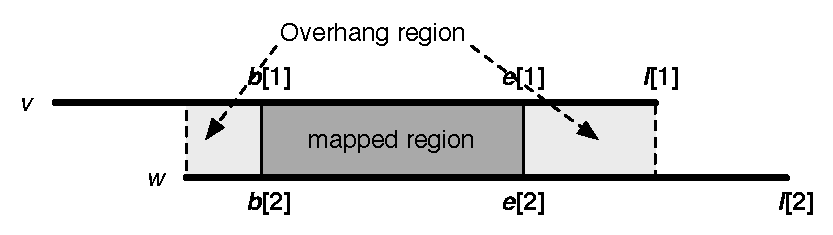
\includegraphics[width=.45\textwidth]{overhang}
\caption{Mapping between two reads. $b[1]$ and $e[1]$ are the starting the
ending mapping coordinates of the first read $v$, respectively. $b[2]$ and
$e[2]$, $b[2]<e[2]$, are the coordiantes on the mapping strand of the second
read $w$. Lightgray areas indicate regions that would be mapped together if the
overlap was perfect. If the overhang regions are small enough, the figure
implies an edge $v\to\overline{w}$ with $\ell(v\to\overline{w})=b[1]-b[2]$ and
an edge $w\to\overline{v}$ with
$\ell(w\to\overline{v})=(l[2]-e[2])-(l[1]-e[1])$.}\label{fig:overhang}
\end{figure}

\begin{algorithm}[ht]
\DontPrintSemicolon
\footnotesize
\KwIn{Read length $l$, mapping begin coordinate $b$ and mapping end $e$ of the
two reads; max overhang length $o$ and max overhang to mapping length ratio
$r$}
\KwOut{hashed $p$-bit integer}
\BlankLine
\textbf{Function} {\sc ClassifyMapping}$(l[2], b[2], e[2], o, r)$
\Begin {
	${\it overhang}\gets\min(b[1], b[2])+\min(l[1]-e[1],l[2]-e[2])$\;
	${\it maplen}\gets\max(e[1]-b[1],e[2]-b[2])$\;
	\uIf{${\it overhang}>\min(o,{\it maplen}\cdot r)$} {
		\Return {\tt INTERNAL\_MATCH}
	} \uElseIf {$b[1]\le b[2]$ {\bf and} $l[1]-e[1]\le l[2]-e[2]$} {
		\Return {\tt FIRST\_CONTAINED}
	}\uElseIf {$b[1]\ge b[2]$ {\bf and} $l[1]-e[1]\ge l[2]-e[2]$} {
		\Return {\tt SECOND\_CONTAINED}
	} \uElseIf {$b[1]>b[2]$} {
		\Return {\tt FIRST\_TO\_SECOND\_OVERLAP}
	} \Else {
		\Return {\tt SECOND\_TO\_FIRST\_OVERLAP}
	}
}
\caption{Mapping classification}
\end{algorithm}

For each trimmed mapping, miniasm applies Algorithm~5 to classify the mapping
(see also Figure~\ref{fig:overhang} for the explanation of input variables).
It ignores internal matches, drops contained reads and adds overlaps to the
assembly graph.


\subsubsection{Graph cleaning}

\begin{algorithm}[ht]
\DontPrintSemicolon
\footnotesize
\KwIn{$G=(V,E)$, starting vertex $v_0$ and maximum probe distance $d$}
\KwOut{the sink vertex of a bubble within $d$; or {\bf nil} if not found}
\BlankLine
\textbf{Function} {\sc DetectBubble}$(V,E,v_0,d)$
\Begin {
	\lIf{$\mathrm{deg}^+(v_0)<2$} { \Return {\bf nil} } \Comment*[r]{Not a source of bubble}
	\lFor{$v\in V$} { $\delta[v]\gets\infty$ } \Comment*[r]{the min distance from $v_0$ to $v$}
	$\delta[v_0]\gets0$\;
	$S\gets$ empty stack \Comment*[r]{Vertices with all incoming edges visited}
	{\sc Push}$(S,v_0)$\;
	$p\gets0$ \Comment*[r]{Number of visited vertices never added to $S$}
	\While{$S$ is not empty} {
		$v\gets$ {\sc Pop}$(S)$\;
		\ForEach{$v\to w\in E$} {
			\If (\Comment*[f]{A circle involving the starting vertex}) {$w=v_0$} {
				\Return {\bf nil}\;
			}
			\If (\Comment*[f]{Moving too far}) {$\delta[v]+\ell(v\to w)>d$} {
				\Return {\bf nil}\;
			}
			\If (\Comment*[f]{Not visited before}) {$\delta[w]=\infty$} {
				$\gamma[w]\gets \mathrm{deg}^-(w)$ \Comment*[r]{No. unvisited incoming edges}
				$p\gets p+1$\;
			}
			\If{$\delta[v]+\ell(v\to w)<\delta[w]$} {
				\nl$\delta[w]\gets \delta[v]+\ell(v\to w)$\;
			}
			$\gamma[w]\gets\gamma[w]-1$\;
			\If (\Comment*[f]{All incoming edges visited}) {$\gamma[w]=0$} {
				\If (\Comment*[f]{Not a tip}) {$\mathrm{deg}^+(w)\not=0$} {
					{\sc Push}$(S,w)$\;
				}
				$p\gets p-1$\;
			}
		}
		\If (\Comment*[f]{Found the sink}) {$|S|=1$ {\bf and} $p=0$} {
			\Return {\sc Pop}$(S)$\;
		}
	}
	\Return {\bf nil}\;
}
\caption{Bubble detection}
\end{algorithm}

After constructing the assembly graph, miniasm removes transitive
edges~\citep{Myers:2005bh}, trims tips and pops small
bubbles~\citep{Zerbino:2008uq}. Algorithm~6 detects bubbles. This algorithm is
adapted from Kahn's topological sorting algorithm~\citep{Kahn62aa}. It starts
from the potential source and visits a vertex when all its incoming edges are
visited before. Algorithm~6 only detects bubbles. We can keep track of the
optimal parent vertex at line~1 and then backtrack to collapse bubbles to a
single path. Fermi~\citep{Li:2012fk} uses a similar algorithm except that it
keeps two optimal paths through the bubble.  \citet{DBLP:conf/wabi/OnoderaSS13}
and \citet{TCS15} have also independently found similar algorithms.

In addition, if $v\to w_1$ and $v\to w_2$ exist and $\ell(v\to w_1)<\ell(v\to
w_2)$, miniasm removes $v\to w_2$ if $[|v|-\ell(v\to w_2)]/[|v|-\ell(v\to
w_1)]$ is small enough (70\% by default). When there are longer overlaps,
shorter overlaps after transitive reduction may be due to repeats.
However, non-repetitive overlaps may also be removed at a small chance, which
leads to missing overlaps and misassemblies.

\subsection{Formats}

\subsubsection{Pairing mapping format (PAF)}

\begin{table}[tb]\label{tab:paf}
\processtable{Pairwise mapping format (PAF)}
{\footnotesize
\begin{tabular}{rcl}
\toprule
Col & Type & Description \\
\midrule
1 & string & Query sequence name \\
2 & int    & Query sequence length \\
3 & int    & Query start coordinate (0-based) \\
4 & int    & Query end coodinate (0-based) \\
5 & char   & `+' if query and target on the same strand; `-' if opposite \\
6 & string & Target sequence name \\
7 & int    & Target sequence length \\
8 & int    & Target start coordinate on the original strand \\
9 & int    & Target end coordinate on the original strand \\
10& int    & Number of matching bases in the mapping \\
11& int    & Number bases, including gaps, in the mapping \\
12& int    & Mapping quality (0--255 with 255 missing unavailable) \\
\botrule
\end{tabular}
}{PAF is TAB-delimited text format with each line consisting of the above fixed
fields. When the alignment is available, column 11 equals the total number of
sequence matches, mismatches and gaps in the alignment. Column 10 divided by
column 11 gives the alignment identity. If the detailed alignment is not
available, column 10 and 11 can be approximate. PAF may optionally have
additional fields in the SAM-like typed key-value format~\citep{Li:2009ys}.}
\end{table}

PAF is a lightweight format keeping the key mapping information (Table~2).
Minimap outputs mappings in PAF, which are taken by miniasm as input for
assembly. We also provide scripts to convert DALIGNER, MHAP and SAM formats to
PAF.

\subsubsection{Graphical fragment assembly format (GFA)}

\begin{table}[tb]
\processtable{Graphical fragment assembly format (GFA)}
{\footnotesize
\begin{tabular}{clp{5.8cm}}
\toprule
Line & Comment & Fixed fields \\
\midrule
H    & Header  & N/A \\
S    & Segment & segName,segSeq \\
L    & Overlap & segName1,segOri1,segName2,segOri2,CIGAR \\
\botrule
\end{tabular}
}{GFA is a line-based TAB-delimited format. Each line starts with a single
letter determining the interpretation of the following TAB-delimited fields. In
GFA, segment refers to a read or a unitig. A line start with `S' gives the name
and sequence of a segment. When the sequence is not available, it can be a star
`*'. Overlaps between segments are represented in lines starting with `L',
giving the names and orientations of the two segments in an overlap. The last
field `CIGAR' on an `L'-line describes the detailed alignment of the overlap if
available. In addition to the types of lines in the table, GFA may contain
other line types starting with different letters. Each line may optionally have
additional SAM-like typed key-value pairs.}
\end{table}

GFA is a concise assembly format (http://bit.ly/gfaspec) initially proposed by
us prior to miniasm and later improved by community (P. Melsted, S.  Jackman,
J. Simpson and E. Garrison, personal communication). It has already been
adopted by a few tools.  Notably, FASTG (http://bit.ly/fastgfmt) is another
assembly format, but it is primarily designed to describe the final assembly
graph, not the intermediate assembly graph. GFA is designed for both types of
graphs.

\end{methods}

\begin{table}[htb]
\processtable{Evaluation data sets}
{\footnotesize
\begin{tabular}{llrrr}
\toprule
Name & Species & Size & Cov. & N50 \\
\midrule
PB-ce-40X     & {\it Caenorhabditis elegans}      & 104M & 45  & 16572 \\
ERS473430     & {\it Citrobacter koseri}          & 4.9M & 106 & 7543  \\
ERS544009     & {\it Yersinia pseudotuberculosis} & 4.7M & 147 & 9002  \\
ERS554120     & {\it Pseudomonas aeruginosa}      & 6.4M & 90  & 7106  \\
ERS605484     & {\it Vibrio vulnificus}           & 5.0M & 155 & 5091  \\
ERS617393     & {\it Acinetobacter baumannii}     & 4.0M & 237 & 7911  \\
ERS646601     & {\it Haemophilus influenzae}      & 1.9M & 258 & 4081  \\
ERS659581     & {\it Klebsiella sp.}              & 5.1M & 129 & 8031  \\
ERS670327     & {\it Shimwellia blattae}          & 4.2M & 155 & 6765  \\
ERS685285     & {\it Streptococcus sanguinis}     & 2.4M & 224 & 5791  \\
ERS743109     & {\it Salmonella enterica}         & 4.8M & 188 & 6051  \\
PB-ecoli      & {\it Escherichia coli}            & 4.6M & 160 & 13976 \\
PBcR-PB-ec    & {\it Escherichia coli}            & 4.6M & 30  & 11757 \\
PBcR-ONT-ec   & {\it Escherichia coli}            & 4.6M & 29  & 9356  \\
MAP-006-1     & {\it Escherichia coli}            & 4.6M & 54  & 10892 \\
MAP-006-2     & {\it Escherichia coli}            & 4.6M & 30  & 10794 \\
MAP-006-pcr-1 & {\it Escherichia coli}            & 4.6M & 30  & 8080  \\
MAP-006-pcr-2 & {\it Escherichia coli}            & 4.6M & 60  & 8064  \\
\botrule
\end{tabular}
}{Evaluation data set name, species, reference genome size, theoretical
sequencing coverage and the N50 read length. Names starting with ``MAP'' are
unpublished recent ONT data provided by the Loman lab (http://bit.ly/loman006).
Names starting with ``ERS'' are accession numbers of unpublished PacBio data
from the NCTC project (http://bit.ly/nctc3k). PB-ecoli and PB-ce-40X are PacBio
public data sets sequenced with the P6/C4 chemistry (http://bit.ly/pbpubdat;
retrieved on 11/03/2015). PBcR-PB-ec is the PacBio sample data (P5/C3
chemistry) used in the tutorial of the PBcR pipeline; PBcR-ONT-ec is the ONT
example originally used by \citet{Loman:2015xu}. `pls2fasta --trimByRegion' was
applied to ERS* and PB-ecoli data sets as they do not provide read sequences in
the FASTQ format.}
\end{table}

\section{Results}

\subsection{Assembling bacterial genomes}

We evaluated the performance of miniasm on 17 bacterial data sets data sets
(Table~4). We used command line `minimap -Sw5 -L100 -m0 reads.fa reads.fa $|$
miniasm -f reads.fa -'. Miniasm is able to derive a single contig per
chromosome/plasmid for all but four data sets: 3 extra $>$50kb contigs for
ERS554120, and 1 extra contig for ERS605484, PBcR-ONT-ec and MAP-006-pcr-1
each. 

Encouraged by the single-contig assembly for PBcR-PB-ec at only 30-fold
coverage, we randomly down-sampled PacBio data sets and tried to assemble the
subset. For PB-ecoli, miniasm still produced a single contig at 24-fold
coverage, or two contigs at 20-fold. For the other data sets, however, miniasm
generated fragmented assemblies when we sampled a third of reads. We speculate
the shorter read lengths of the ERS* data sets made it more difficult to
produce good assemblies at relatively low coverage.

We have also run the PBcR pipeline~\citep{Berlin:2015xy}. PBcR reqires a spec
file. We took `pacbio.spec' and `oxford.spec' from PBcR-PB-ec and PBcR-ONT-ec,
respectively, and applied them to all data sets based on their data types. MAP*
data sets only provide FASTA sequences for download. We assigned quality 9 to
all bases as PBcR requires base quality. PBcR assembled all PacBio data sets
without extra contigs longer than 50kb -- better than miniasm. However, on the
ONT data sets, PBcR produced more fragmented assemblies for MAP-006-2,
MAP-006-pcr-1 and MAP-006-pcr-2, and deleted a 300kb region for the PBcR-ONT-ec
data set. 

With four CPU cores, it took miniasm 13 seconds to assemble the 30-fold
PBcR-PB-ec data set and 2 minutes to assemble the 160-fold PB-ecoli data set.
PBcR, with four CPU cores, too, is about 60 times slower on PB-ecoli and 700
times slower on PBcR-PB-ec.  The performance is worse on low-coverage input
because PBcR automatically switches to the slower sensitive mode. Here we
should remind readers that without an error correction stage, the contig
sequences generated by miniasm are of much lower accuracy in comparison to
PBcR. The speed comparison is not fair. Nonetheless, miniasm is still tens of
times faster than PBcR excluding the time spent on error correction.

\subsection{Assembling a C. elegans genome}

\begin{figure}[tb]
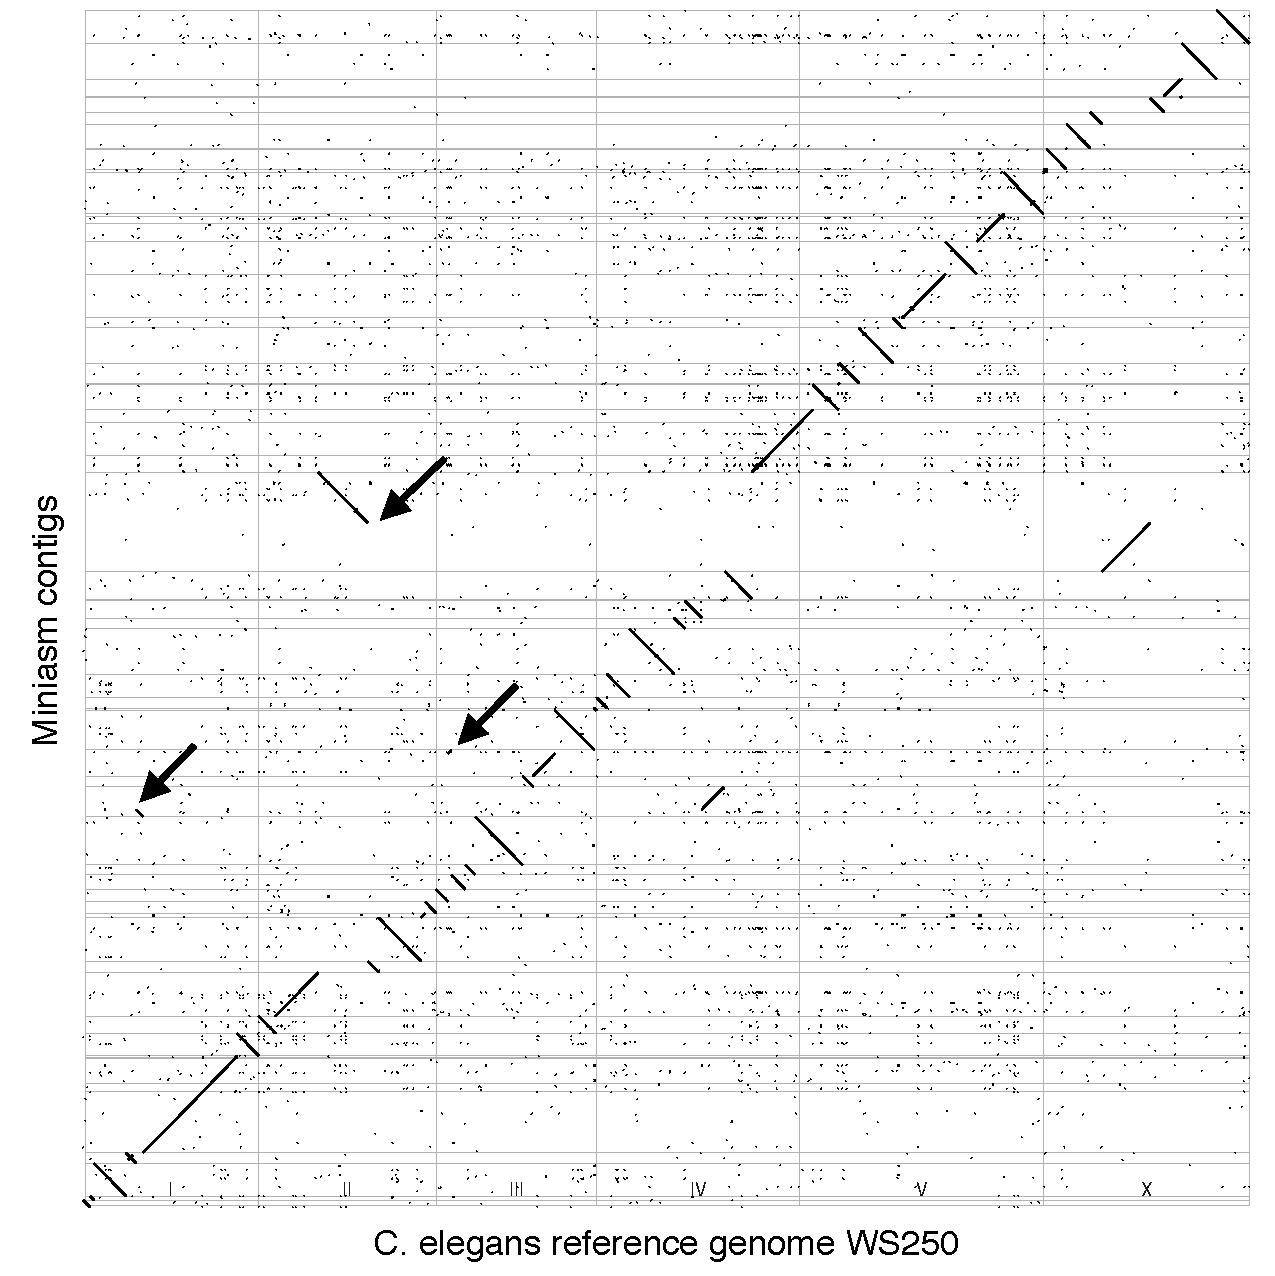
\includegraphics[width=.48\textwidth]{ce}
\caption{Dotter plot comparing the miniasm assembly and the {\it C. elegans}
reference genome. Thin gray lines are boundaries of contigs or chromosomes. The
three arrows indicate large-scale misassemblies visible from the
plot. The mapping is done by minimap.}\label{fig:ce}
\end{figure}

We assembled a 45-fold {\it C. elegans} data set (Table~4). With 16 CPU cores,
miniasm assembled the data in 9 minutes, achieving an N50 size 2.8Mb. From the
dotter plot (Figure~\ref{fig:ce}), we observed three large-scale misassemblies
(readers are advised to zoom into the vector graph to see the details).  Due to
the high per-base error rate of the miniasm contigs, we have not been able to
produce realible whole-genome alignment to analyze local misassemblies in a
satisfactory manner.

PacBio has assembled the same data set with HGAP3~\citep{Chin:2013qr}. The
dotter plot between the {\it C. elegans} reference genome and the HGAP3
assembly shows no visible large-scale misassemblies, though the N50 is shorter
(1.6Mb).

We have also tried PBcR on this data set. Based on the intermediate progress
report, we estimated that with 16 CPU cores, it would take a week or so to
finish the assembly in the automatically chosen `sensitive' mode.

\bibliography{miniasm}
\end{document}
